\documentclass[9pt,twoside]{pnas-new}
% Use the lineno option to display guide line numbers if required.

\templatetype{pnasmathematics} % Choose template 
% {pnasresearcharticle} = Template for a two-column research article
% {pnasmathematics} = Template for a one-column mathematics article
% {pnasinvited} = Template for a PNAS invited submission

%remove watermark
\setboolean{displaywatermark}{false}

\title{Topological  Fractal  Dimension  of  Networks  of Protein–Protein  Interaction  Networks}
%PNAS LaTeX Template for preparing single-column mathematics articles on Overleaf
% Use letters for affiliations, numbers to show equal authorship (if applicable) and to indicate the corresponding author
\author[a]{Georgios Kalantzis}
\author[a]{Andrei Stoica} 

\affil[a]{SABS, DTC}

% Please give the surname of the lead author for the running footer
%\leadauthor{Lead author last name} 

% Please add here a significance statement to explain the relevance of your work
\significancestatement{Authors must submit a 120-word maximum statement about the significance of their research paper written at a level understandable to an undergraduate educated scientist outside their field of speciality. The primary goal of the Significance Statement is to explain the relevance of the work in broad context to a broad readership. The Significance Statement appears in the paper itself and is required for all research papers.}

% Please include corresponding author, author contribution and author declaration information
%\authorcontributions{Please provide details of author contributions here.}
%\authordeclaration{Please declare any conflict of interest here.}
%\equalauthors{\textsuperscript{1}A.O.(Author One) and A.T. (Author Two) contributed equally to this work (remove if not applicable).}
%\correspondingauthor{\textsuperscript{2}To whom correspondence should be addressed. E-mail: author.two\@email.com}

% Keywords are not mandatory, but authors are strongly encouraged to provide them. If provided, please include two to five keywords, separated by the pipe symbol, e.g:
\keywords{Keyword 1 $|$ Keyword 2 $|$ Keyword 3 $|$ ...} 

\begin{abstract}
Please provide an abstract of no more than 250 words in a single paragraph. Abstracts should explain to the general reader the major contributions of the article. References in the abstract must be cited in full within the abstract itself and cited in the text.
\end{abstract}

\dates{This manuscript was compiled on \today}
%\doi{\url{www.pnas.org/cgi/doi/10.1073/pnas.XXXXXXXXXX}}

\begin{document}

\maketitle
\thispagestyle{firststyle}
\ifthenelse{\boolean{shortarticle}}{\ifthenelse{\boolean{singlecolumn}}{\abscontentformatted}{\abscontent}}{}

% If your first paragraph (i.e. with the \dropcap) contains a list environment (quote, quotation, theorem, definition, enumerate, itemize...), the line after the list may have some extra indentation. If this is the case, add \parshape=0 to the end of the list environment.
\dropcap{T}his PNAS journal template is provided for authors to use when writing a mathematics article in a single column format. Instructions are provided below.



\subsection*{Author Affiliations}

Include department, institution, and complete address, with the ZIP/postal code, for each author. Use lower case letters to match authors with institutions, as shown in the example. Authors with an ORCID ID may supply this information at submission.

\subsection*{Submitting Manuscripts}

All authors must submit their articles at \href{http://www.pnascentral.org/cgi-bin/main.plex}{PNAScentral}. If you are using Overleaf to write your article, you can use the ``Submit to PNAS'' option in the top bar of the editor window. 

\subsection*{Format}

Please be sure to include: Title, Author Affiliations, Keywords, Abstract, Significance, Statement, Acknowledgments, and References. Other sections and headings are permitted as need.

\subsection*{Manuscript Length}

The maximum length of a Direct Submission research article is six pages and a Direct Submission Plus research article is ten pages including all text, spaces, and the number of characters displaced by figures, tables, and equations.  When submitting tables, figures, and/or equations in addition to text, keep the text for your manuscript under 39,000 characters (including spaces) for Direct Submissions and 72,000 characters (including spaces) for Direct Submission Plus.

\subsection*{References}

References should be cited in numerical order as they appear in text; this will be done automatically via bibtex, e.g. \cite{belkin2002using} and \cite{berard1994embedding,coifman2005geometric}. All references should be included in the main manuscript file. 

\subsection*{Data Archival}

PNAS must be able to archive the data essential to a published article. Where such archiving is not possible, deposition of data in public databases, such as GenBank, ArrayExpress, Protein Data Bank, Unidata, and others outlined in the Information for Authors, is acceptable.

\subsection*{Language-Editing Services}
Prior to submission, authors who believe their manuscripts would benefit from professional editing are encouraged to use a language-editing service (see list at www.pnas.org/site/authors/language-editing.xhtml). PNAS does not take responsibility for or endorse these services, and their use has no bearing on acceptance of a manuscript for publication. 

\begin{figure}%[tbhp]
\centering
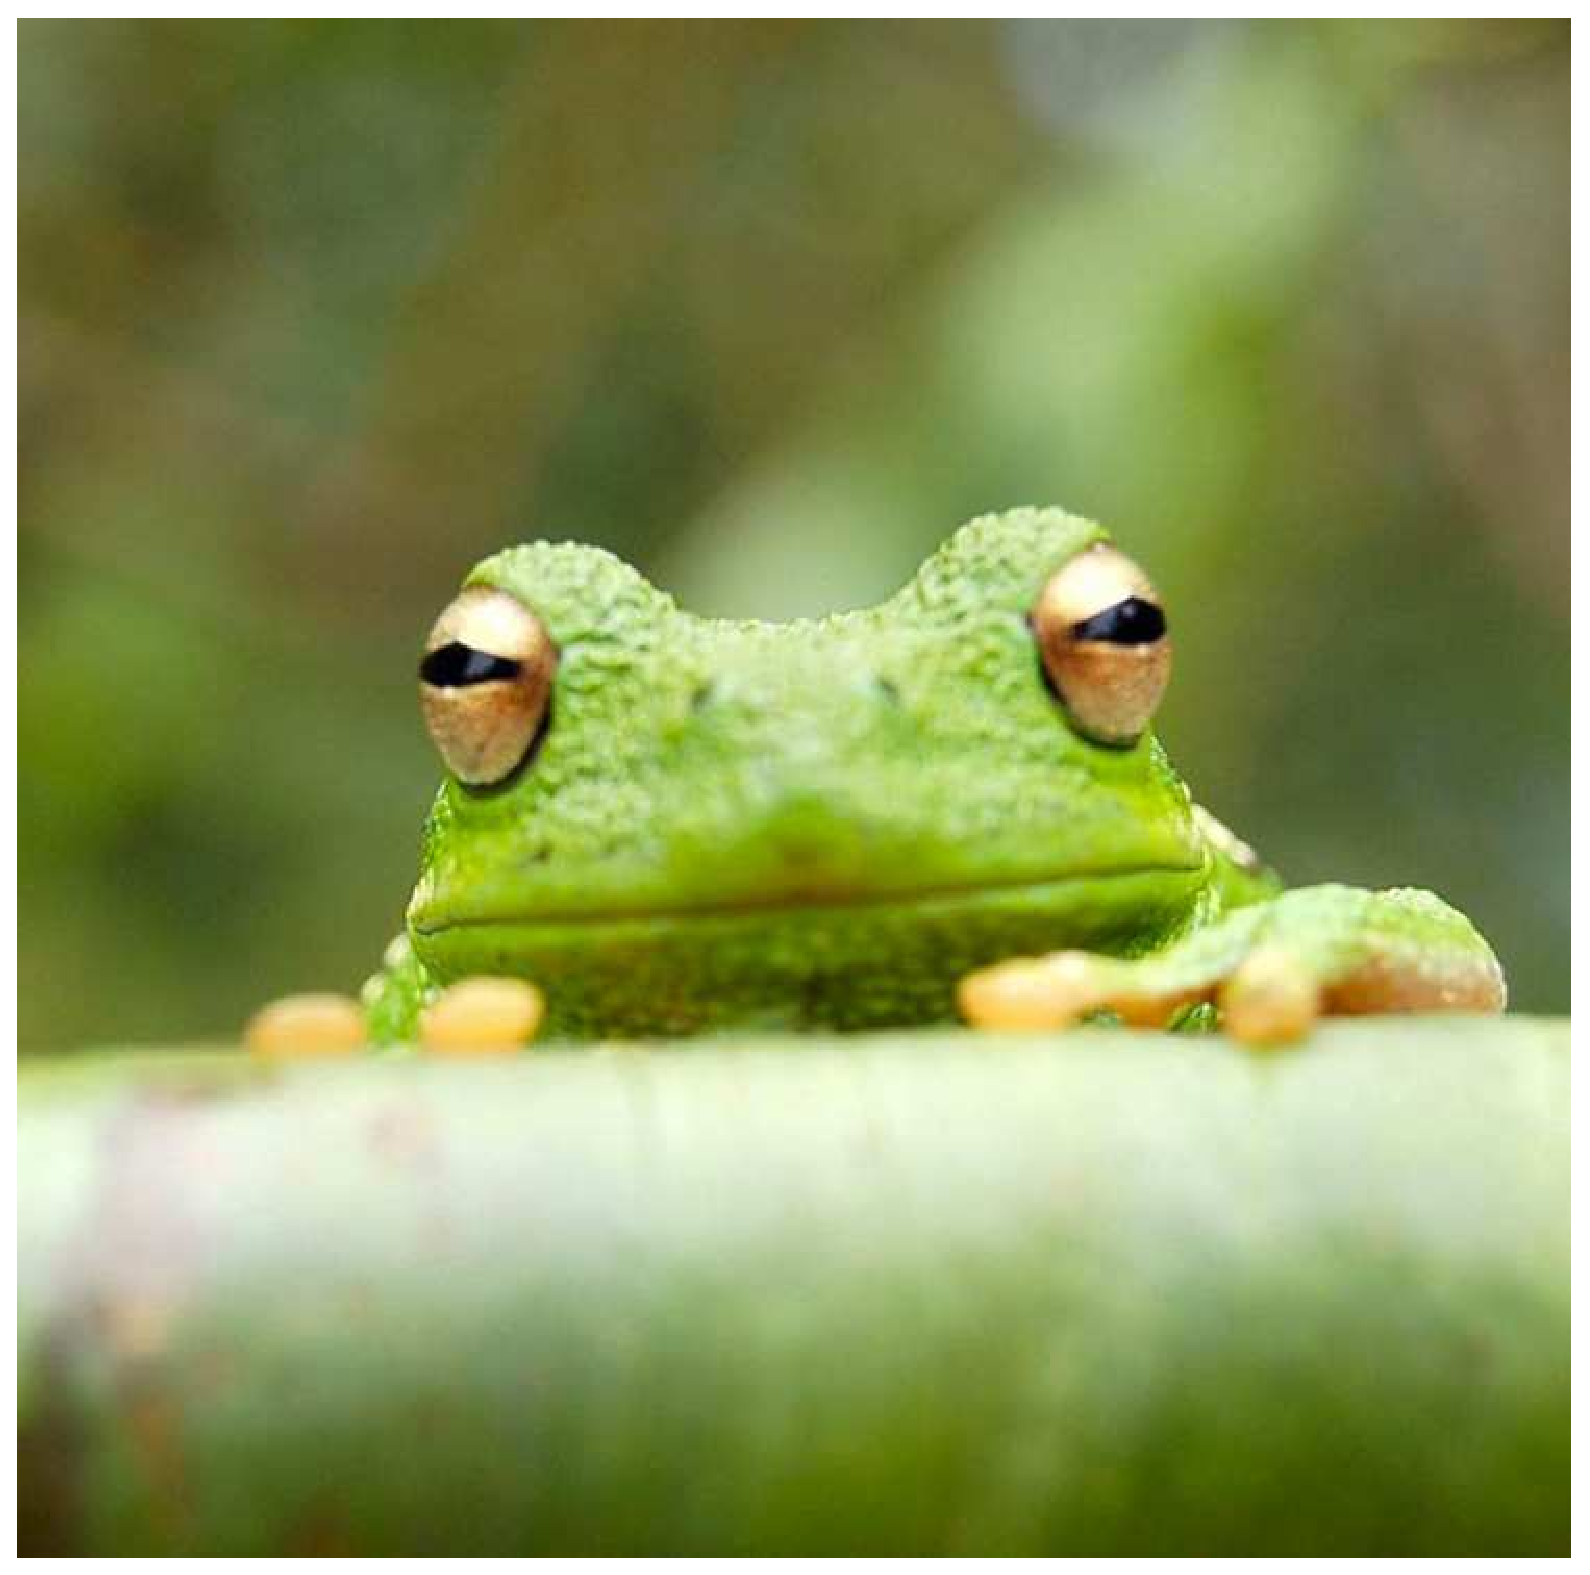
\includegraphics[width=.5\linewidth]{frog}
\caption{Placeholder image of a frog with an example caption.}
\label{fig:frog}
\end{figure}


\begin{SCfigure*}[\sidecaptionrelwidth][t]
\centering
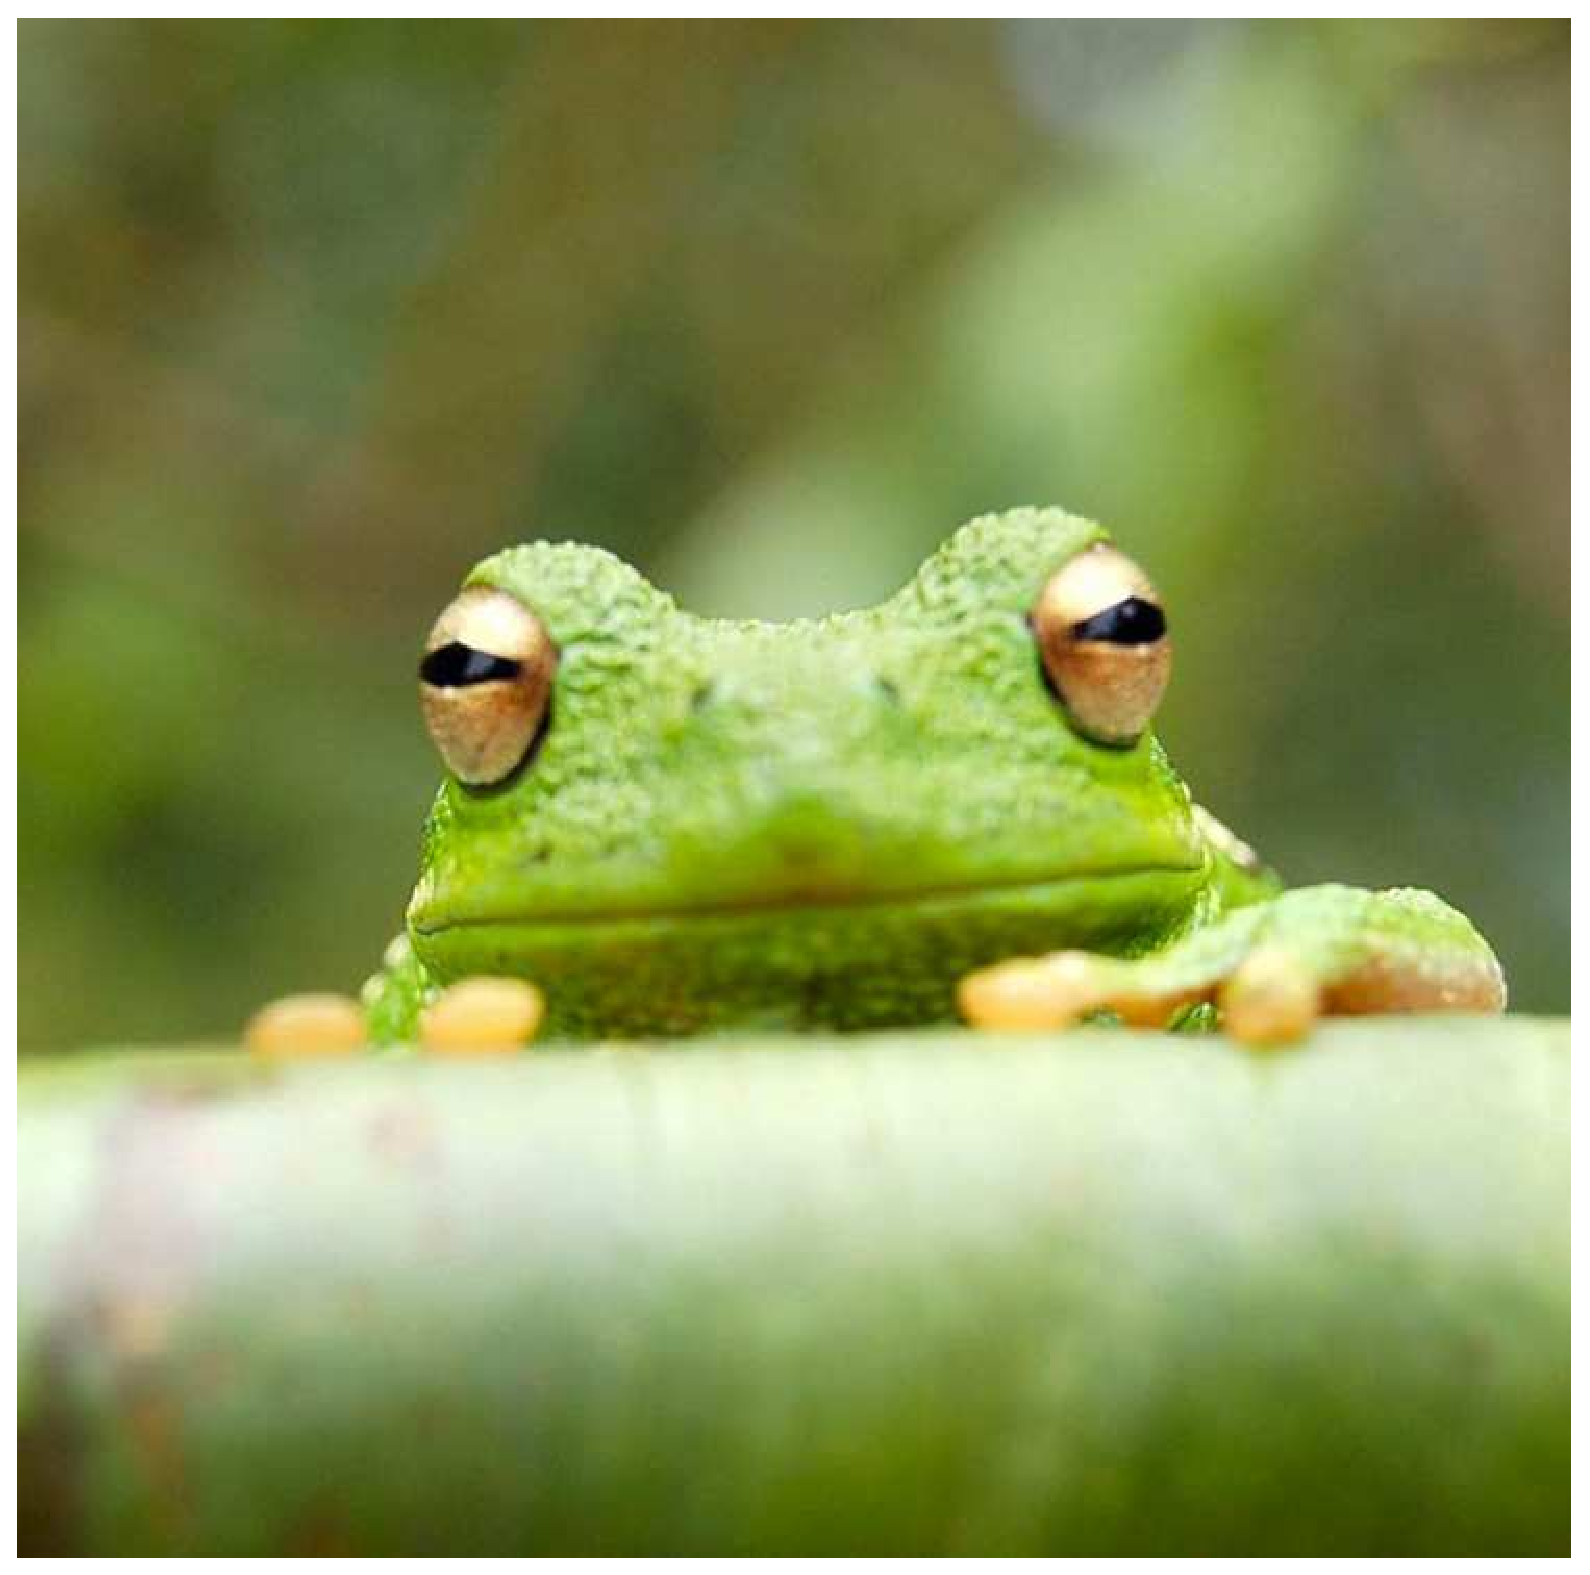
\includegraphics[width=11.4cm,height=11.4cm]{frog}
\caption{This caption would be placed at the side of the figure, rather than below it.}\label{fig:side}
\end{SCfigure*}


\subsection*{Digital Figures}
Only TIFF, EPS, and high-resolution PDF for Mac or PC are allowed for figures that will appear in the main text, and images must be final size. Authors may submit U3D or PRC files for 3D images; these must be accompanied by 2D representations in TIFF, EPS, or high-resolution PDF format.  Color images must be in RGB (red, green, blue) mode. Include the font files for any text. 

Figures and Tables should be labelled and referenced in the standard way using the \verb|\label{}| and \verb|\ref{}| commands.

Figure \ref{fig:frog} and Table \ref{tab:energy} show examples of how to insert figures and tables respectively.

\begin{table}%[tbhp]
\centering
\caption{Comparison of the fitted potential energy surfaces and ab initio benchmark electronic energy calculations}
\begin{tabular}{lrrr}
Species & CBS & CV & G3 \\
\midrule
1. Acetaldehyde & 0.0 & 0.0 & 0.0 \\
2. Vinyl alcohol & 9.1 & 9.6 & 13.5 \\
3. Hydroxyethylidene & 50.8 & 51.2 & 54.0\\
\bottomrule
\end{tabular}

\addtabletext{nomenclature for the TSs refers to the numbered species in the table.}
\label{tab:energy}
\end{table}


\subsection*{Tables}
In addition to including your tables within this manuscript file, PNAS requires that each table be uploaded to the submission separately as a “Table” file.  Please ensure that each table .tex file contains a preamble, the \verb|\begin{document}| command, and the \verb|\end{document}| command. This is necessary so that the submission system can convert each file to PDF.

\subsection*{Supporting Information (SI)}

Authors should submit SI as a single separate PDF file, combining all text, figures, tables, movie legends, and SI references.  PNAS will publish SI uncomposed, as the authors have provided it.  Additional details can be found here: \href{http://www.pnas.org/page/authors/journal-policies}{policy on SI}.  For SI formatting instructions click \href{https://www.pnascentral.org/cgi-bin/main.plex?form_type=display_auth_si_instructions}{here}.  The PNAS Overleaf SI template can be found \href{https://www.overleaf.com/latex/templates/pnas-template-for-supplementary-information/wqfsfqwyjtsd}{here}.  Refer to the SI Appendix in the manuscript at an appropriate point in the text. Number supporting figures and tables starting with S1, S2, etc.

Authors who place detailed materials and methods in an SI Appendix must provide sufficient detail in the main text methods to enable a reader to follow the logic of the procedures and results and also must reference the SI methods. If a paper is fundamentally a study of a new method or technique, then the methods must be described completely in the main text.

\subsubsection*{SI Datasets} 

Supply Excel (.xls), RTF, or PDF files. This file type will be published in raw format and will not be edited or composed.


\subsubsection*{SI Movies}

Supply Audio Video Interleave (avi), Quicktime (mov), Windows Media (wmv), animated GIF (gif), or MPEG files and submit a brief legend for each movie in a Word or RTF file. All movies should be submitted at the desired reproduction size and length. Movies should be no more than 10 MB in size.


\subsubsection*{3D Figures}

Supply a composable U3D or PRC file so that it may be edited and composed. Authors may submit a PDF file but please note it will be published in raw format and will not be edited or composed.

\acknow{Please include your acknowledgments here, set in a single paragraph. Please do not include any acknowledgments in the Supporting Information, or anywhere else in the manuscript.}

\showacknow % Display the acknowledgements section
\def\rownumber{} % hack for re-starting row-counter (and skip the header) 
\begin{table}[h] %[tbhp]
	\centering
	\caption{\textit{Appendix} - Basic Information about PPINs from \texttt{BioGrid 3.5.165 dataset}}
	\label{table:stats}
    \begin{tabular}{@{\makebox[2em][r]{\rownumber\space}} | lrrcccr}
		\textbf{Organism} & \textbf{\# Nodes} &  \textbf{\# Edges} & \textbf{Avg Degree} & \textbf{ConComps} & \textbf{Largest} & \textbf{Diam} %[0.5ex] 
        \gdef\rownumber{\stepcounter{magicrownumbers}\arabic{magicrownumbers}} \\
		\midrule
        $ Anopheles \ gambiae \ PEST $ & 2 & 1 & 1.00 & 1 & 1.000 & 1 \\ 
        $ Apis \ mellifera $ & 2 & 1 & 1.00 & 1 & 1.000 & 1 \\ 
        $ Arabidopsis \ thaliana \ Columbia $ & 9570 & 35242 & 7.37 & 78 & 0.981 & 12 \\ 
        $ Bacillus \ subtilis \ 168 $ & 2 & 1 & 1.00 & 1 & 1.000 & 1 \\ 
        $ Bos \ taurus $ & 437 & 405 & 1.85 & 73 & 0.162 & 15 \\ 
        $ Caenorhabditis \ elegans $ & 3938 & 7885 & 4.00 & 77 & 0.953 & 13 \\ 
        $ Candida \ albicans \ SC5314 $ & 713 & 860 & 2.41 & 30 & 0.893 & 12 \\ 
        $ Canis \ familiaris $ & 52 & 34 & 1.31 & 20 & 0.135 & 4 \\ 
        $ Cavia \ porcellus $ & 9 & 5 & 1.11 & 4 & 0.333 & 2 \\ 
        $ Chlamydomonas \ reinhardtii $ & 19 & 15 & 1.58 & 4 & 0.632 & 2 \\ 
        $ Chlorocebus \ sabaeus $ & 11 & 7 & 1.27 & 4 & 0.273 & 2 \\ 
        $ Cricetulus \ griseus $ & 32 & 24 & 1.50 & 8 & 0.500 & 3 \\ 
        $ Danio \ rerio $ & 245 & 250 & 2.04 & 37 & 0.404 & 8 \\ 
        $ Dictyostelium \ discoideum \ AX4 $ & 24 & 18 & 1.50 & 6 & 0.208 & 2 \\ 
        $ Drosophila \ melanogaster $ & 9191 & 54806 & 11.93 & 37 & 0.992 & 9 \\ 
        $ Emericella \ nidulans \ FGSC \ A4 $ & 64 & 62 & 1.94 & 6 & 0.703 & 2 \\ 
        $ Equus \ caballus $ & 4 & 2 & 1.00 & 2 & 0.500 & 1 \\ 
        $ Escherichia \ coli \ K12 $ & 2 & 1 & 1.00 & 1 & 1.000 & 1 \\ 
        $ Escherichia \ coli \ K12 \ MC4100 \ BW2952 $ & 10 & 8 & 1.60 & 2 & 0.800 & 6 \\ 
        $ Escherichia \ coli \ K12 \ MG1655 $ & 146 & 127 & 1.74 & 21 & 0.623 & 3 \\ 
        $ Escherichia \ coli \ K12 \ W3110 $ & 4063 & 181620 & 89.40 & 1 & 1.000 & 5 \\ 
        $ Gallus \ gallus $ & 391 & 417 & 2.13 & 42 & 0.588 & 9 \\ 
        $ Glycine \ max $ & 44 & 39 & 1.77 & 7 & 0.318 & 2 \\ 
        $ Hepatitus \ C \ Virus $ & 131 & 129 & 1.97 & 2 & 0.985 & 2 \\ 
        $ Homo \ sapiens $ & 22826 & 318912 & 27.94 & 14 & 0.999 & 9 \\ 
        $ Human \ Herpesvirus \ 1 $ & 174 & 194 & 2.23 & 1 & 1.000 & 8 \\ 
        $ Human \ Herpesvirus \ 2 $ & 7 & 4 & 1.14 & 3 & 0.429 & 2 \\ 
        $ Human \ Herpesvirus \ 3 $ & 4 & 2 & 1.00 & 2 & 0.500 & 1 \\ 
        $ Human \ Herpesvirus \ 4 $ & 240 & 235 & 1.96 & 7 & 0.771 & 8 \\ 
        $ Human \ Herpesvirus \ 5 $ & 91 & 79 & 1.74 & 12 & 0.385 & 4 \\ 
        $ Human \ Herpesvirus \ 6A $ & 11 & 7 & 1.27 & 4 & 0.364 & 2 \\ 
        $ Human \ Herpesvirus \ 6B $ & 7 & 4 & 1.14 & 3 & 0.429 & 2 \\ 
        $ Macaca \ mulatta $ & 15 & 12 & 1.60 & 3 & 0.733 & 2 \\ 
        $ Human \ Herpesvirus \ 7 $ & 2 & 1 & 1.00 & 1 & 1.000 & 1 \\ 
        $ Meleagris \ gallopavo $ & 2 & 1 & 1.00 & 1 & 1.000 & 1 \\ 
        $ Human \ Immunodeficiency \ Virus \ 1 $ & 1121 & 1299 & 2.32 & 1 & 1.000 & 5 \\ 
        $ Human \ Immunodeficiency \ Virus \ 2 $ & 16 & 12 & 1.50 & 4 & 0.500 & 4 \\ 
        $ Human \ papillomavirus \ 16 $ & 14 & 12 & 1.71 & 2 & 0.857 & 4 \\ 
        $ Mus \ musculus $ & 13003 & 38624 & 5.94 & 89 & 0.984 & 15 \\ 
        $ Neurospora \ crassa \ OR74A $ & 12 & 10 & 1.67 & 2 & 0.667 & 2 \\ 
        $ Mycobacterium \ tuberculosis \ H37Rv $ & 11 & 9 & 1.64 & 2 & 0.818 & 2 \\ 
        $ Nicotiana \ tomentosiformis $ & 2 & 1 & 1.00 & 1 & 1.000 & 1 \\ 
        $ Oryctolagus \ cuniculus $ & 283 & 271 & 1.92 & 33 & 0.502 & 9 \\ 
        $ Oryza \ sativa \ Japonica $ & 74 & 90 & 2.43 & 18 & 0.351 & 3 \\ 
        $ Pan \ troglodytes $ & 10 & 5 & 1.00 & 5 & 0.200 & 1 \\ 
        $ Ovis \ aries $ & 2 & 1 & 1.00 & 1 & 1.000 & 1 \\ 
        $ Pediculus \ humanus $ & 2 & 1 & 1.00 & 1 & 1.000 & 1 \\ 
        $ Plasmodium \ falciparum \ 3D7 $ & 1224 & 2445 & 4.00 & 23 & 0.963 & 10 \\ 
        $ Rattus \ norvegicus $ & 3713 & 5227 & 2.82 & 118 & 0.918 & 14 \\ 
        $ Ricinus \ communis $ & 3 & 2 & 1.33 & 1 & 1.000 & 2 \\ 
        $ Saccharomyces \ cerevisiae \ S288c $ & 7158 & 534073 & 149.22 & 1 & 1.000 & 6 \\ 
        $ Schizosaccharomyces \ pombe \ 972h $ & 4292 & 58217 & 27.13 & 7 & 0.997 & 8 \\ 
        $ Selaginella \ moellendorffii $ & 6 & 8 & 2.67 & 1 & 1.000 & 2 \\ 
        $ Simian \ Immunodeficiency \ Virus $ & 19 & 16 & 1.68 & 4 & 0.421 & 3 \\ 
        $ Simian \ Virus \ 40 $ & 6 & 5 & 1.67 & 1 & 1.000 & 2 \\ 
        $ Solanum \ lycopersicum $ & 45 & 96 & 4.27 & 7 & 0.467 & 4 \\ 
        $ Solanum \ tuberosum $ & 4 & 2 & 1.00 & 2 & 0.500 & 1 \\ 
        $ Sus \ scrofa $ & 94 & 79 & 1.68 & 23 & 0.234 & 5 \\ 
        $ Strongylocentrotus \ purpuratus $ & 17 & 16 & 1.88 & 1 & 1.000 & 2 \\ 
        $ Vaccinia \ Virus $ & 8 & 5 & 1.25 & 3 & 0.375 & 2 \\ 
        $ Tobacco \ Mosaic \ Virus $ & 3 & 2 & 1.33 & 1 & 1.000 & 2 \\ 
        $ Ustilago \ maydis \ 521 $ & 4 & 3 & 1.50 & 1 & 1.000 & 2 \\ 
        $ Xenopus \ laevis $ & 1128 & 1212 & 2.15 & 61 & 0.850 & 15 \\ 
        $ Vitis \ vinifera $ & 2 & 1 & 1.00 & 1 & 1.000 & 1 \\ 
        $ Zea \ mays $ & 21 & 11 & 1.05 & 10 & 0.143 & 2 \\ 
        $ Human \ Herpesvirus \ 8 $ & 714 & 687 & 1.92 & 45 & 0.529 & 12 \\ 
                %[1ex] 
		\bottomrule
    \end{tabular}
	%\addtabletext{nomenclature for the TSs refers to the numbered species in the table.}
\end{table}
% Bibliography
\bibliography{pnas-sample}

\end{document}